\pdfoutput=1
\documentclass[11pt]{article}
\usepackage{emnlp2023}
\usepackage{times}
\usepackage{latexsym}
\usepackage[T1]{fontenc}
\usepackage[utf8]{inputenc}
\usepackage{microtype}
\usepackage{inconsolata}
\usepackage{graphicx}
\usepackage{booktabs}
\usepackage{amsmath}
\usepackage{capt-of}
\usepackage{array}

% Float placement: let full-width tables share the top of a page with text, and
% tighten the space around floats and captions, so columns don't end in gaps.
\renewcommand{\topfraction}{0.9}
\renewcommand{\dbltopfraction}{0.9}
\renewcommand{\bottomfraction}{0.8}
\renewcommand{\textfraction}{0.07}
\renewcommand{\floatpagefraction}{0.85}
\renewcommand{\dblfloatpagefraction}{0.85}
\setcounter{topnumber}{3}
\setcounter{dbltopnumber}{3}
\setcounter{totalnumber}{5}
\setlength{\floatsep}{6pt plus 2pt minus 2pt}
\setlength{\dblfloatsep}{6pt plus 2pt minus 2pt}
\setlength{\textfloatsep}{8pt plus 2pt minus 2pt}
\setlength{\dbltextfloatsep}{8pt plus 2pt minus 2pt}
\setlength{\abovecaptionskip}{4pt}
\setlength{\belowcaptionskip}{0pt}
% Let columns end short rather than stretch the space between paragraphs and headings.
\raggedbottom

\title{ReAgent: Closed-Loop Self-Healing for Open-Weight Tool-Calling Agents, from Structural Hallucinations to Decision Errors}

\author{Charlie Galvin  \quad Katie Kitchen \quad Chiara Picardi \\
  Lloyds Banking Group \\
  \texttt{\{charlie.galvin,katie.kitchen,chiara.picardi\}@lloydsbanking.com}}

\begin{document}
\maketitle

\begin{abstract}
When language-model agents can modify databases, hallucinations manifest as erroneous actions. Untuned, Aya Expanse 32B solves 14.5\% of $\tau^2$-bench's customer-service test tasks, and 95\% of its conversations invoke an unavailable tool, fabricate an argument or repeat a failed call. We present ReAgent, a closed loop in which a rule-based classifier localises failures, an open-weight teacher supplies corrections verified by the benchmark, QLoRA retrains the student, and a pre-registered gate decides whether the updated adapter is deployed. On held-out tasks, hallucinated conversations fall from 95\% to 10\% and task success rises to 51.5\%; run autonomously, the gate rejects an adapter that hallucinates less but solves no additional tasks. The residual failures are decision errors, which neither our detectors nor reinforcement learning corrected. Extending training on the same verified data did: task success reached 60.0\% ($+9.9$ points, 95\% CI $+3.9$ to $+16.0$), comparable to GPT-4.1 (61.5\%) at under a third of its cost per conversation, while state changes made without the customer's consent fell from 0.152 to 0.010 per conversation and general capability was preserved. Code, data and adapters are available at \url{https://github.com/CharlieGalvin/lexsi-labs-reflexive-agent}.
\end{abstract}

\begin{figure*}[t]
\centering
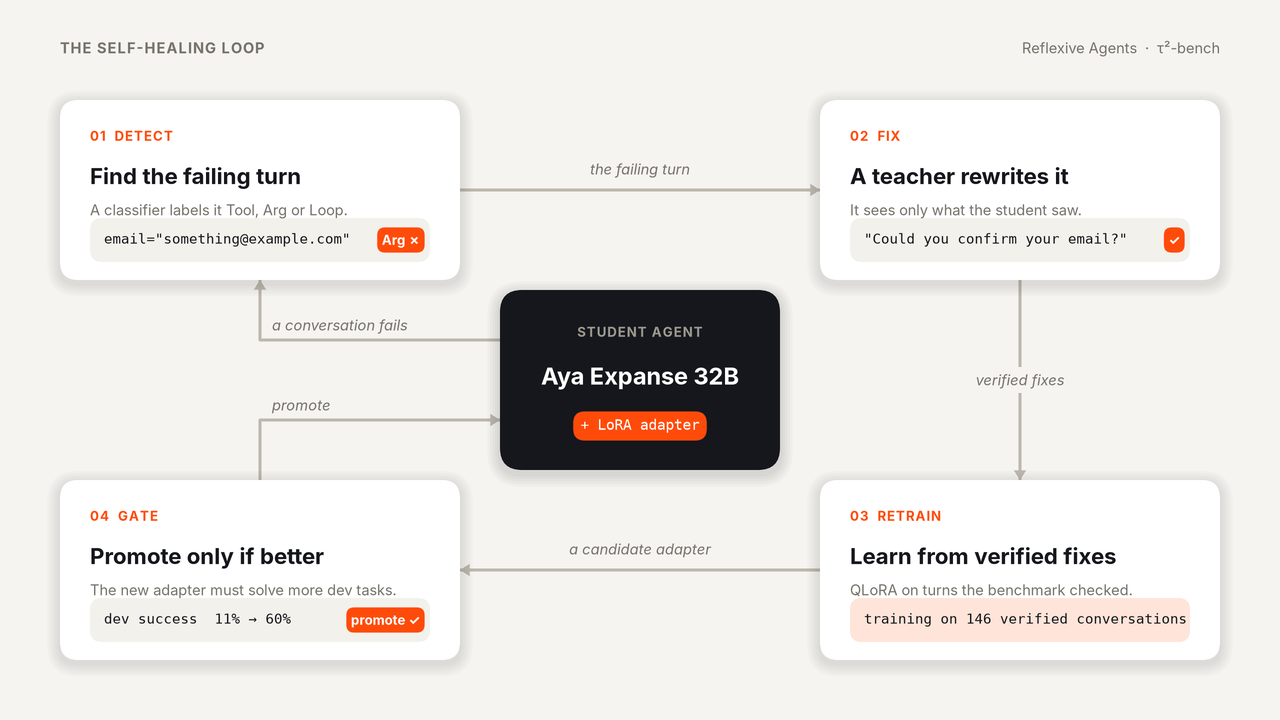
\includegraphics[width=0.92\textwidth]{figures/heal-loop.png}
\caption{Overview of the Detect--Fix--Retrain--Gate loop. The gate example shows the healed model's dev result (11\% $\rightarrow$ 60\%) after training on 146 verified conversations.}
\label{fig:loop}
\end{figure*}

\section{Introduction}
\label{sec:intro}

Customer-service agents increasingly perform consequential actions, such as cancelling orders, rebooking flights and modifying accounts. In benchmarks that model such settings, including $\tau$-bench and $\tau^2$-bench \citep{Yao2024TauBench,Barres2025Tau2Bench}, every tool call alters the environment state, so a hallucinated argument modifies the wrong record. Organisations that deploy open-weight models on their own infrastructure, such as Aya Expanse 32B \citep{Dang2024AyaExpanse} served with vLLM \citep{Kwon2023EfficientMemory}, require reliability that these models lack out of the box. Aya solves 14.5\% of $\tau^2$-bench's test tasks, and 95.0\% of its conversations contain a hallucinated tool or argument: it invokes phone tools available only to the customer, submits placeholders such as \texttt{email="something@example.com"}, and retries calls that have already failed. A prompt enumerating each of these errors leaves success at 13.0\%, which suggests that the behaviour is encoded in the weights and must be corrected there.

We propose ReAgent, a \textbf{Detect $\rightarrow$ Fix $\rightarrow$ Retrain $\rightarrow$ Gate} loop (Figure~\ref{fig:loop}). A deterministic classifier identifies the turn at which a conversation first fails and labels the error as \textbf{Tool}, \textbf{Arg} or \textbf{Loop}. An open-weight teacher, GLM-5.3-Flash, selected from 12 candidates, supplies a correction that is retained only if $\tau^2$-bench verifies it. QLoRA \citep{Dettmers2023QLoRA} retrains the student on the verified corrections, and a gate, \texttt{DevGate}, determines on 36 development (dev) tasks whether the new adapter replaces the current one.

The study proceeded in two stages, each evaluated against decision rules recorded before the corresponding runs (Stage~2's are dated in \texttt{docs/experiments/STAGE2.md}). Stage~1 addresses four research questions: whether fine-tuning on verified teacher conversations reduces hallucination on unseen tasks (RQ1); whether prompting suffices (RQ2); whether the loop can operate autonomously and promote only improved adapters (RQ3); and whether reinforcement learning yields further gains (RQ4). Stage~2, conducted after the first test evaluation, asks whether a checker without access to the answer key can identify the remaining decision errors and whether blocking them improves success (RQ5), whether healing degrades general capability (RQ6), and, after observing that v2 failed half of its own training tasks, whether it was under-trained (RQ7). Data splits were frozen before training, and three test arms were declared before the Stage~1 evaluation: \textbf{A}, the untuned model; \textbf{C}, the untuned model with a prompt enumerating every failure type; and \textbf{B}, the healed model, SFT v2. The first fine-tuned version, SFT v1, was trained on 112 verified teacher conversations; v2 adds 34 airline conversations (\S\ref{sec:exp_ablations}).

\paragraph{Related work.}\label{sec:related_work} Our work builds on $\tau^2$-bench's environments and uses its evaluator to determine success. FireAct \citep{Chen2023FireAct} and AgentTuning \citep{Zeng2023AgentTuning} showed that open models can acquire agentic behaviour from the trajectories of stronger models; we additionally verify every trajectory and gate every adapter. As in DAgger \citep{Ross2011DAgger}, an expert corrects the states the learner actually visits; in contrast to Reflexion \citep{Shinn2023Reflexion}, which corrects an agent in context, we update its weights. Our attempt to improve further with GRPO (Group Relative Policy Optimization; \citealp{Shao2024DeepSeekMath}) resulted in reward hacking \citep{Skalse2022RewardHacking}: the policy learned to obtain reward without completing the task.

This work addresses Track~3 (Agentic Fine-tuning): \#8 Self-healing agents (main); \#2 Efficient trajectories (steps per task 24.8 $\rightarrow$ 19.2, redundant calls halved); \#1 Reliable tool calling (by SFT on verified rollouts; reinforcement learning attempted); \#3 Agentic distillation (into a 32B student served in FP8 on one GPU); and \#9 Reward design and reward-hacking defences (a negative result).

\section{Methodology}
\label{sec:method}

\subsection{Failure Taxonomy}
\label{sec:method_taxonomy}

In each $\tau^2$-bench task, the agent serves a simulated customer under a written policy $p_d$ for its domain $d$ (retail, airline or telecom), using agent tools with JSON schemas; in telecom, the customer also has phone tools, which the agent must ask them to operate. A conversation $\tau$ is a sequence of customer messages $u_t$, agent turns $a_t$ and tool results $o_t$ over $T$ turns,
\begin{equation}
\tau = \big(p_d, u_1, a_1, o_1, \dots, u_T, a_T, o_T\big),
\end{equation}
and succeeds, $V(\tau)=1$, only if the database ends in exactly the state the task requires and, where the benchmark specifies, the agent communicated the required information. $V$ is $\tau^2$-bench's evaluator, and every test verdict is re-scored by the outcome oracle of AuditKIT, Lexsi Labs' evaluation suite \citep{Arora2026AuditKIT}; Appendix~\ref{app:submission} describes how the Lexsi Labs kits connect. Learning from failures requires identifying them cheaply and consistently; our classifier $\mathcal{C}$ is therefore rule-based rather than an LLM judge. Operating only on information available to the agent, it checks each turn for 12 error kinds grouped into three families (Appendix~\ref{app:rubric}). A \textbf{Tool} error invokes a tool unavailable to the agent, most often a customer-side phone tool such as \texttt{check\_network\_status}. An \textbf{Arg} error supplies a value the agent could not have known: a placeholder such as \texttt{"YYYY-MM-DD"}, an ID or email absent from the conversation, or a value that violates the schema. A \textbf{Loop} repeats a failed call, issues the same call or reply three or more times, or reaches the 200-step limit. The earliest such turn, $t^*$, defines the point at which the teacher intervenes. A separate runtime monitor, \texttt{no\_progress}, flags three consecutive repeated text-only turns (Appendix~\ref{app:tables}).

\subsection{The Self-Healing Loop}
\label{sec:method_loop}

ReAgent iterates four steps, either manually or autonomously on a single GPU (Figure~\ref{fig:loop}). In \textbf{Detect}, the current model is run on the training tasks (test tasks are excluded by construction), and the classifier records each failure's findings and $t^*$. In \textbf{Fix}, the teacher repairs a failure at one of two granularities, a distinction that proves consequential. At the \emph{turn level}, it rewrites turn $t^*$ only, and the rewrite is accepted if the classifier detects no error; at the \emph{trajectory level}, it re-executes the entire task, and the conversation is retained only if $\tau^2$-bench judges it successful. In the latter mode, the outcome verifier determines the training data, while the classifier diagnoses failures and informs the gate. In \textbf{Retrain}, Aya \citep{Dang2024AyaExpanse} is fine-tuned on the verified corrections with QLoRA \citep{Dettmers2023QLoRA} (rank 16, 4-bit; 95.7M trainable parameters, 0.30\% of its weights), with the loss computed over agent tokens only:
\begin{multline}
\mathcal{L}_{\text{SFT}}(\phi) = -\frac{1}{\sum_{i=1}^N |\mathcal{M}_i|} \sum_{i=1}^N \sum_{j \in \mathcal{M}_i} \\
\log \pi_{\theta_0 + \Delta\theta(\phi)}\!\left(x_{i,j} \mid x_{i,<j}\right),
\end{multline}
where $x_1,\dots,x_N$ are the $N$ verified conversations, $\mathcal{M}_i$ the positions of the agent's tokens in $x_i$, $\theta_0$ Aya's frozen weights and $\Delta\theta(\phi)$ the LoRA update with parameters $\phi$. Consequently, a turn-level correction supervises approximately 1\% of a conversation's tokens, whereas a trajectory supervises all agent turns. In \textbf{Gate}, a candidate replaces the current adapter only if, on 36 frozen dev tasks re-scored by AuditKIT, the run is complete (at most two crashes), the candidate wins at least two more tasks than it loses relative to the current adapter, its hallucination findings per conversation increase by at most 10\%, and no domain loses two or more tasks (Table~\ref{tab:gate_rules}). At most three decisions may be taken on the same dev tasks, which prevents the gate from being exhausted by repeated attempts; a candidate that passes is deployed to the live server.

\subsection{Reinforcement Learning Variants}
\label{sec:method_grpo}
Reinforcement learning could reward the student directly for avoiding the errors the classifier identifies. We evaluate GRPO \citep{Shao2024DeepSeekMath}, implemented in AgentTune, Lexsi Labs' post-training library \citep{Lyngkhoi2026AgentTune}, from SFT v2: the policy samples 8 candidate turns per conversation prefix, with a KL penalty ($\beta=0.04$) towards SFT v2. \textbf{Arm G} scores tool-call turns against the teacher's call. \textbf{Arm H} trains on the 178 points at which base Aya first failed, with one reward per failure type (no unavailable tool, no fabricated argument, no repetition) and one for agreement with the teacher's correction, applied only when the sampled turn has the teacher's type (call or reply). \textbf{Arm H2} adds a reward that verifies each write call against the actions the task still requires (details in Appendix~\ref{app:kit_settings}).

\subsection{Stage 2: Detecting and Blocking Made-Up Intent}
\label{sec:method_stage2}
Stage~1's classifier assesses how an action is formed, not whether the customer requested it. Stage~2 therefore introduces a fourth finding type, \emph{made-up intent}: a state change the customer did not request, or one executed before the customer consented to it. Its rules access only the conversation and the policy, never $\tau^2$-bench's expected actions (enforced by a test), and were frozen before any validation run. The \textbf{no-yes} rule flags a state-changing call executed without the customer's explicit consent to that change: a lexical match is applied first, and candidate violations are passed to a GPT-4.1-mini judge whose affirmative verdict is accepted only if it quotes the customer. Because the telecom policy requires confirmation only for data top-ups, the rule is restricted there to \texttt{refuel\_data}. The \textbf{mismatch} rule asks GPT-4.1 whether a change made with one of seven retail and airline tools deviates from the customer's request or from the results of the agent's own lookups. We also evaluated \emph{meta-healing}, in which GPT-4.1 proposes rules from v2's unexplained failures, and a \emph{hybrid judge} that reads a complete conversation with programmatically computed facts. The \textbf{guard} applies the frozen rules at run time: before a state-changing call reaches $\tau^2$-bench, a finding blocks the reply, and the agent is re-prompted with a fixed instruction to describe the change and request the customer's confirmation. Blocks are capped per change (2) and per conversation (10).

\section{Experiments}
\label{sec:experiments}

\subsection{Setup}
\label{sec:exp_setup}

We use $\tau^2$-bench v2.0.0 \citep{Barres2025Tau2Bench}: 278 English tasks across retail, airline and telecom, with GPT-4.1 simulating the customer. Aya's failures are behavioural rather than mechanical: none of its 266 replies in a 30-task review was malformed, yet it completed only 1 of 30 database-modifying tasks. Of the 142 training tasks, 112 constitute the \emph{healable pool} (tasks that base Aya fails and the teacher solves) and 30 form a validation set, used solely to select between SFT versions under predefined rules; the 36 dev tasks are reserved for the gate, and the 100 test tasks were evaluated once per declared arm, with two samples per task. Splits are disjoint by exact task ID, and every script that reads conversations for training or analysis refuses test task IDs (\texttt{assert\_not\_test}). Each adapter is trained with Hugging Face TRL in under 30 minutes on a single H100 (Appendices~\ref{app:hyperparams} and~\ref{app:kit_settings}). Arms A and C (prompt in Appendix~\ref{app:prompts}) are served through Cohere's API with a 128K context; B and all other adapters are served with vLLM 0.33 \citep{Kwon2023EfficientMemory} with a 32K context, as is a fourth arm, \textbf{P}, the untuned model on the same server, which isolates the effect of training from that of serving. We report task success, the proportion of conversations containing a Tool/Arg hallucination or a loop, AuditKIT's tool-call validity (the proportion of calls to an existing tool with schema-valid arguments), latency and output length, with 95\% task-level bootstrap confidence intervals and exact McNemar tests.

\subsection{Teacher Selection and Classifier Validation}
\label{sec:exp_teacher}

We screened 12 candidate teachers on 30 database-modifying training tasks (Table~\ref{tab:bakeoff_full}, Appendix~\ref{app:bakeoff}). The four strongest (Qwen3.8 27B 30/30, Claude Sonnet 5.5 29/30, GLM-5.3-Flash and DeepSeek V4 Flash 27/30) were statistically indistinguishable (Holm-corrected exact McNemar, $p = 1.00$), yet their projected costs ranged from \$12 to \$182; Aya itself completed only 1 of 30 tasks and was outperformed by every teacher ($p \le 0.002$). Across all 178 non-test tasks, GLM-5.3-Flash succeeded on 88\% at the first attempt and yielded verified solutions for 158 tasks at a cost of \$11.20, and was therefore adopted as the teacher. A manual inspection of 30 classifier findings (10 per type) found all correct (95\% CI 72--100\% per type) and explains the failure of the careful prompt: $\tau^2$-bench's telecom manual describes customer phone actions in function-call syntax (\texttt{check\_network\_status()}), which Aya executes directly. The prompt consequently left the number of customer-tool calls essentially unchanged (412 vs.\ 422).

\subsection{Held-Out Results}
\label{sec:exp_test}

\begin{table*}[t]
\centering
\footnotesize
\setlength{\tabcolsep}{4pt}
\resizebox{\textwidth}{!}{%
\begin{tabular}{lccccccc}
\toprule
\textbf{Arm} & \textbf{Success (95\% CI)} & \textbf{Retail} & \textbf{Airline} & \textbf{Telecom} & \textbf{Tool/Arg Halluc.} & \textbf{Loop (Cls.)} & \textbf{Tool Valid.} \\
\midrule
\textbf{A}: Untuned Aya 32B & 14.5\% (9.5--20.0) & 12.5\% & 17.5\% & 15.0\% & 95.0\% (92.0--98.0) & 49.0\% (42.0--56.0) & 72.2\% \\
\textbf{C}: Careful Prompt & 13.0\% (7.5--19.0) & 10.0\% & 20.0\% & 12.5\% & 95.5\% & 49.5\% & 75.3\% \\
\textbf{B}: Healed (SFT v2) & \textbf{51.5\%} (43.5--59.5) & \textbf{60.0\%} & \textbf{30.0\%} & \textbf{53.8\%} & \textbf{10.0\%} (6.0--14.5) & \textbf{27.0\%} (21.0--33.5) & \textbf{97.6\%} \\
\midrule
\multicolumn{8}{l}{\textit{Diagnostics (B vs.\ A):} Seconds per agent request, median (mean), 2.4 (2.8) vs.\ 3.3 (3.7) (C: 3.5 (3.7))$^\dagger$; median output tokens 78 vs.\ 117 (C: 117);} \\
\multicolumn{8}{l}{Tool validity: Retail 100\% vs.\ 98.8\%, Airline 99.9\% vs.\ 97.7\%, Telecom 94.1\% vs.\ 32.8\%.} \\
\bottomrule
\end{tabular}%
}
\caption{Held-out $\tau^2$-bench test results (100 tasks $\times$ 2 samples = 200 conversations/arm; all 600 oracle-verified by AuditKIT with 0 disagreements; 95\% task-level bootstraps). $^\dagger$Arm B runs self-hosted on vLLM/H100 (32K context; 2/200 overflows scored as failures) while A and C run on Cohere's API (128K), so latency reflects serving differences.}
\label{tab:main_test}
\end{table*}

Table~\ref{tab:main_test} addresses RQ1 and RQ2. Trained on 146 verified teacher conversations, the healed agent B solves 51.5\% of test tasks, compared with 14.5\% for the untuned agent, a paired gain of 37.0 points (95\% CI $+28.0$ to $+45.5$), with improvements in every domain, largest in retail (12.5\% to 60.0\%). The careful prompt yields 13.0\% ($-1.5$ points, 95\% CI $-7.0$ to $+4.0$), and hallucinations persist in 95.5\% of conversations, indicating that explicit instruction does not alter the behaviour. Against P, served identically to B, the gain persists on dev (11\% to 60\%, $p=0.0001$) and validation (9.0 to 17.0 of 30). Hallucinations are largely eliminated: conversations containing a hallucinated tool or argument decrease from 95.0\% to 10.0\%, loops from 49.0\% to 27.0\%, and tool-call validity increases from 72.2\% to 97.6\%, almost entirely in telecom (32.8\% to 94.1\%), where the untuned agent repeatedly invoked customer-side tools. Validity alone would not capture most of the problem: in retail, 98.8\% of the untuned agent's calls were already valid, since a fabricated email address is still a well-formed string; only a grounding check, which verifies that each value appeared earlier in the conversation, detects it. The healed agent also produces shorter turns (78 vs.\ 117 tokens), although conversations lengthen (25.6 steps per task). Appendix~\ref{app:cases} presents a retail return before and after healing.

\subsection{Autonomous Healing Cycles}
\label{sec:exp_cycles}

To address RQ3, we executed the full loop autonomously on a single H100 twice, starting from base Aya and using the same gate: Cycle~1 with turn-level and Cycle~2 with trajectory-level corrections (Table~\ref{tab:auto_cycles}, Appendix~\ref{app:tables}). In Cycle~1, on 30 sampled training tasks, the teacher repaired all 24 fixable failures, mostly at turn 3 by requesting the customer's identity instead of guessing it. Trained on 16 such turns, the resulting adapter reduced hallucination findings on dev by 71\% but solved no additional tasks (4 of 36 before and after), and the gate rejected it; a deployment criterion based on hallucination rates alone would have accepted it. In Cycle~2, trained on complete conversations for all 112 training tasks, the adapter reduced findings by 87\% and increased dev success from 6 to 22 of 36 (17 wins, 1 loss; $p=0.0001$); the gate promoted it, and the loop deployed it to the live server without human intervention. As the cycles also differ in pool size, deduplication and training steps, and Cycle~2 drew on v2's training pool, this shows that the loop can reproduce v2's promotion autonomously; the held-out evidence remains B's test result.

\subsection{Ablations, Reward Hacking and Residual Errors}
\label{sec:exp_ablations}

Table~\ref{tab:sft_grpo} (Appendix~\ref{app:tables}) reports every SFT version against the predefined rules. SFT v1, trained on 112 verified conversations, eliminated all Tool/Arg findings on dev and raised success from 11\% to 38\%, but the gate rejected it because it lost two airline tasks, mostly by cancelling ineligible bookings. Adding 34 verified airline conversations produced SFT v2, which reached 60\% on dev and passed the gate. Three further variants (SL, v1's data for v2's steps; v3, more retail data; v4, corrections of v2's own errors) scored 15.5--17.0 of 30 on validation, below the adoption threshold of 19.5. Reinforcement learning did not improve on SFT v2 either (RQ4), because the policies exploited their rewards. Arm G ceased to address the customer, repeating the same lookup 1,850 times across 24 telecom runs, and scored 0.5 of 30. Arm H improved every structural measure (findings per conversation fell from 1.17 to 0.25), yet its dev success fell from 60\% to 51\% and the gate rejected it: the rewards assigned full credit to a valid call with a real ID regardless of whether the customer had requested the action, and the policy cancelled 12 airline bookings without any request. Arm H2, which added a reward for the correct state change, was terminated early by its drift guard (14.5 of 30). After healing, the residual failures are predominantly decision errors. Almost all of base Aya's dev failures began with an early Tool or Arg error, whereas 37 of SFT v2's 55 failed dev and validation conversations contain no classifier finding (Tables~\ref{tab:failure_shift} and~\ref{tab:val_causes}): the agent omits a required state change, misapplies an airline rule or skips a telecom step. This accounts for the persistently low success in airline (30.0\%), the most rule-intensive domain, and motivates Stage~2.

\subsection{Stage 2: Decision Errors and Extended Training}
\label{sec:exp_stage2}

\begin{table}[t]
\centering
\footnotesize
\setlength{\tabcolsep}{2pt}
\begin{tabular}{@{}lccc@{}}
\toprule
\textbf{Arm} & \textbf{Val} & \textbf{Test} & \textbf{$\Delta$ vs.\ v2 (95\% CI)} \\
\midrule
A: untuned, API$^\ast$ & --- & 14.5\% & --- \\
P: untuned, vLLM$^\ast$ & 9.0 & 11.5\% & --- \\
B: SFT v2 & 16.0 & 50.1\% & --- \\
\textbf{v2-E4} & \textbf{18.5} & \textbf{60.0\%} & $\mathbf{+9.9}$ ($+3.9$, $+16.0$) \\
v2-E4+practice & 17.9 & 58.9\% & $+8.8$ ($+3.6$, $+13.9$) \\
\midrule
GPT-4.1 (reference)$^\ast$ & --- & 61.5\% & --- \\
\bottomrule
\end{tabular}
\caption{Stage~2 results. Val: validation tasks solved (of 30). Test: task success on the 100 test tasks. All arms use eight samples per task except those marked $^\ast$ (two). v2's first two test samples correspond to its Stage~1 run (51.5\%, Table~\ref{tab:main_test}). $\Delta$: gain over v2 in percentage points, with a paired task-level bootstrap 95\% CI. GPT-4.1 also simulates the customer.}
\label{tab:stage2}
\end{table}

Table~\ref{tab:stage2} and this subsection address RQ5--RQ7. Our detectors identified that a conversation had failed, but rarely where. Applied once by a team member who did not develop it, the frozen checker flagged only 6 of the 37 decision failures above (16\%, 95\% CI 8--31\%) and 2 of the 77 successful conversations. A human audit of the 37 (one labeller, one main error each) shows why: the main error was a reasoning slip in 27 (misreading a tool result, wrong arithmetic, the wrong item or an early transfer) and a policy violation in 8, with 2 unclear; in none was it an unrequested or unconfirmed change, the errors the checker targets (0 of 37, 95\% CI 0--9\%). Evaluated against $\tau^2$-bench's answer key on 224 previously unseen training-task conversations, no detector satisfied both requirements of the loop. The Tool/Arg/Loop rules identified 56\% of failures but never the turn at which the failure originated (0 of 52); the consent checker located that turn in 15 of the 28 failures it flagged but identified only 27\% of failures; and the hybrid judge identified 42\% and located the turn in 11 of 44. Each detector also flagged 8--14\% of successful conversations, and meta-healing accepted no rule in either of its two versions. Blocking flagged changes likewise yielded no improvement: with the guard active, v2 solved 15.0 of 30 validation tasks, compared with 17.0 without it, and the guard was rejected under the predefined rule. It blocked only 5 replies, in 2 of 60 conversations, and never a change that $\tau^2$-bench expected in a successful conversation. Corrections at \emph{mismatch}'s flags produced only 21 verified conversations, below the 30 required for retraining.

The improvement came instead from recognising that the agent was under-trained. v2 solved only 55 of the 112 training tasks on which it had been trained, although its data contained a verified solution for each, and its held-out loss was still decreasing at the end of training. Because validation with two samples was too noisy (v2's individual samples ranged from 12 to 19 of 30), we moved to eight samples and, before scoring any candidate, fixed an adoption rule: a gain of at least 2.0 tasks, a paired 95\% interval above zero, and no domain decreasing by more than 1.5 tasks. \textbf{v2-E4}, v2's recipe trained for four epochs instead of two, gained 2.5 tasks on validation, but its interval ($-0.75$ to $+5.88$) included zero; it therefore failed the rule and was evaluated on test as a declared additional arm. With two samples, its test gain was $+8.0$ points ($-1.0$ to $+16.5$). We subsequently extended both v2 and v2-E4 to eight samples; because this decision was taken after observing the first result, the nominal 5\% false-positive rate is somewhat optimistic. With eight samples, v2-E4 solves 60.0\% of test tasks, compared with 50.1\% for v2 ($+9.9$ points, 95\% CI $+3.9$ to $+16.0$; the six additional samples alone yield $+10.5$). The gain is consistent across training, validation and test tasks: $+4$, $+2.0$ and $+9.3$ tasks in telecom (51.9\% to 75.0\% on test) and $-2$, $-0.9$ and $0.0$ in retail. It is larger on unseen test tasks than on the training tasks (55 to 60 of 112), indicating improved generalisation rather than memorisation. It arises mainly from fewer unexpected state changes (failed validation conversations containing one decreased from 65 to 52); Appendix~\ref{app:cases} presents an example that v2 failed in all 8 runs and v2-E4 passed in 6. AuditKIT's oracle reproduced $\tau^2$-bench's totals exactly (401 and 480 of 800), its redundant-call rate fell from 16.2\% to 7.2\%, and steps per task fell from 24.8 to 19.2 ($-5.6$, 95\% CI $-7.4$ to $-3.9$). Self-generated practice data added nothing: 100 verified conversations from v2's own attempts (74 tasks), trained for four epochs, yielded 58.9\%, 1.1 points below v2-E4 ($-6.6$ to $+4.4$). Extended training also improved safety without degrading general capability. v2-E4 performed a state change without the customer's consent in 6 of 800 test conversations (0.010 findings per conversation, averaged over tasks, compared with 0.152 for v2; difference $-0.142$, 95\% CI $-0.310$ to $-0.035$), and neither v2 nor v2-E4 dropped on IFEval, GSM8K or Global-MMLU-Lite under our predefined rule (no paired 95\% interval lies entirely below zero; Table~\ref{tab:retention}). In FP8, its weights occupy 32.2 rather than 60.4\,GiB and the context doubles to 64K; test success held (57.8\% vs.\ 60.0\%, $-2.2$, 95\% CI $-6.6$ to $+2.1$; a declared check whose rule was recorded after the run), although loops and redundant calls increased. On our H100, v2-E4 costs about \$0.068 per conversation and \$0.11 per solved task, against \$0.235 and \$0.38 for GPT-4.1: \$68 against \$235 per 1,000 conversations (Table~\ref{tab:latency_cost}). Finally, the untuned model scored 11.5\% on our server and 14.5\% through Cohere's API ($-8.0$ to $+1.5$), so B's gain is not attributable to serving.

\section{Conclusion}
\label{sec:conclusion}
We have shown that an open-weight agent that hallucinates actions can be healed. Prompting had no effect, whereas \$11.20 of verified teacher conversations and under 30 minutes of QLoRA training reduced hallucinated conversations from 95.0\% to 10.0\% and raised test success to 51.5\%. Stage~1 shows that a deployment gate must evaluate outcomes (ours rejected an adapter that reduced hallucination findings by 71\% without solving additional tasks), that corrections must cover entire conversations (4 vs.\ 22 of 36 dev tasks), and that rewards assessing only the form of an action are exploited. Stage~2 addressed the residual decision errors and yields a fourth finding: a self-healing loop can correct only the errors it can localise. Instead, verifying whether the model had learned its existing training data proved decisive: doubling the training reached 60.0\%, comparable to GPT-4.1 (61.5\%). Finally, evaluation needs sufficient samples: with one or two per task, the same model varied by 7 tasks in 30.

\section*{Limitations}
Evidence is limited to one benchmark (100 English test tasks), one student model and three general-capability benchmarks. The v2-E4 gain rests on a single training run (a second seed was not completed), was evaluated on test without meeting our validation rule, and was extended to eight samples after a borderline result; GPT-4.1 is an unpaired two-sample reference. The loop is bounded by its teacher (158 of 178 non-test tasks solved) and requires a simulated customer and an outcome verifier. Some comparisons are confounded: the autonomous cycles differ in more than correction granularity, SL was not run on dev, and every adapter used seed 0. Reinforcement learning was tested only with single-turn rewards, constrained decoding was not a baseline, and classifier recall was not measured; the audit of the 37 had one labeller, so no agreement between labellers is reported.

\section*{Ethics Statement}
Released adapters and data inherit Aya Expanse 32B's CC BY-NC 4.0 licence. The first draft was generated with PaperOrchestra (\texttt{gemini-4-neon}) and revised by the authors with Claude Code (Claude Opus 5.5), which also wrote most of the code under the authors' review.

\section*{Acknowledgements}
We thank Lloyds Banking Group for the GPU credits, Lexsi Labs for running the AI Safety \& Alignment Hackathon and for AgentTune and AuditKIT, and the authors of $\tau^2$-bench, TRL and vLLM.

\bibliography{references}
\bibliographystyle{acl_natbib}

\clearpage
\appendix
\renewcommand{\arraystretch}{1.15}


\section{Prompts, Classifier Rubric, and Deployment Gate Specification}
\label{app:rubric}

\subsection{Agent Prompts}
\label{app:prompts}
Arms A (untuned) and B (healed SFT v2) use $\tau^2$-bench's standard domain agent prompt unchanged. Arm C (\texttt{careful/v1}) appends the following verbatim anti-hallucination instruction block:
\begin{quote}\small\ttfamily
Be careful not to hallucinate:\\
- Only call tools you have been given. Never invent a tool or a tool name.\\
- Only use argument values (IDs, names, dates, amounts) that the user gave you or that a tool returned earlier in this conversation. If you don't have a value, ask the user or look it up first. Never guess or make one up.\\
- If a tool call returns an error, read it and change something before trying again. Never repeat the same call with the same arguments.\\
- Only tell the user things that the policy or a tool result supports. If you don't know, say so.
\end{quote}

\subsection{Tool / Arg / Loop Classifier Rubric}
Table~\ref{tab:rubric} specifies all three classes and 12 failure kinds detected by \texttt{reflexive.hallucination}. During retail validation, we fixed a false-positive rule in which the substring \texttt{"example"} flagged legitimate $\tau^2$-bench customer emails ending in \texttt{@example.com}; the placeholder detector now matches \texttt{"for example"} instead (covered by a regression test), and catches underscore/CamelCase placeholders (e.g., \texttt{customer\_id\_from\_search}, \texttt{CustomerIDfromPreviousToolResult}) and masked dates (\texttt{19XX-05-14}). Note that \texttt{unknown\_param}, \texttt{missing\_param}, and \texttt{wrong\_type} are exercised by unit tests and did not occur in the telecom spot-check rollouts.

\begin{table}[h]
\centering
\footnotesize
\setlength{\tabcolsep}{2.5pt}
\begin{tabular}{llp{3.1cm}}
\toprule
\textbf{Class} & \textbf{Kind} & \textbf{Detection Criterion} \\
\midrule
TOOL & \texttt{customer\_tool} & Calls telecom customer-only phone tool unavailable to agent \\
TOOL & \texttt{unknown\_tool} & Calls tool name not in any schema \\
\midrule
ARG & \texttt{placeholder} & Dummy string (e.g., \texttt{"YYYY-MM-DD"}, \texttt{"customer\_id from..."}) \\
ARG & \texttt{ungrounded} & ID, name, phone, email, or DOB absent from prior turns/outputs \\
ARG & \texttt{unknown\_param} & Parameter name not in tool schema \\
ARG & \texttt{missing\_param} & Required schema parameter omitted \\
ARG & \texttt{wrong\_type} & Argument value violates schema type \\
ARG & \texttt{malformed} & Non-JSON args or unparseable \texttt{Action:} block \\
\midrule
LOOP & \texttt{repeated\_failed\_call} & Re-issues a call that previously errored \\
LOOP & \texttt{repeated\_call} & Same call issued $\ge 3$ times \\
LOOP & \texttt{repeated\_message} & Same agent reply emitted $\ge 3$ times (incl.\ post-handoff) \\
LOOP & \texttt{step\_limit} & Terminated at the 200-step cap \\
\bottomrule
\end{tabular}
\caption{Complete 12-kind structural hallucination classifier rubric (\texttt{reflexive.hallucination}).}
\label{tab:rubric}
\end{table}

\subsection{Sequential DevGate Specification}
Table~\ref{tab:gate_rules} lists the pre-registered sequential deployment gate checks (\texttt{configs/gate.yaml}) evaluated on all 36 frozen dev tasks with AuditKIT oracle re-scoring.

\begin{table}[h]
\centering
\footnotesize
\setlength{\tabcolsep}{4pt}
\begin{tabular}{lp{4.8cm}}
\toprule
\textbf{Check} & \textbf{Pre-Registered Rule} \\
\midrule
1. Complete run & All 36 dev tasks run; $\le 2$ crashes per adapter; else no decision \\
2. Pass rate & Candidate-only passes minus current-only passes $\ge +2$ \\
3. Hallucination & Mean Tool+Arg+Loop findings/conv rises by $\le 10\%$ \\
4. Domains & No domain (retail, airline, telecom) loses $\ge 2$ tasks net \\
Budget & At most 3 gate decisions on the same dev tasks (\texttt{max\_cycles: 3}) \\
\bottomrule
\end{tabular}
\caption{Pre-registered sequential four-check \texttt{DevGate} rules.}
\label{tab:gate_rules}
\end{table}

\section{Complete Hyperparameters, Teacher Bake-off, and Diagnostic Tables}
\label{app:tables}

\subsection{Training Hyperparameters}
\label{app:hyperparams}
Table~\ref{tab:hyperparams} reports the exact training settings and single-H100 runtimes for all SFT and GRPO experiments.

\begin{table*}[t]
\centering
\footnotesize
\setlength{\tabcolsep}{4.5pt}
\begin{tabular}{llrrlr}
\toprule
\textbf{Run} & \textbf{Training data} & \textbf{Steps} & \textbf{Batch} & \textbf{Runtime} & \textbf{Train / val loss} \\
\midrule
SFT v1 & 112 conversations & 56 & $1 \times 4$ & 23 min (54 GB) & 0.450 / 0.393 \\
SFT v2 (Arm B) & 146 conversations & 74 & $1 \times 4$ & 28 min & 0.426 / 0.368 \\
SL (ablation) & 112 conversations & 74 & $1 \times 4$ & 31 min & 0.401 / 0.365 \\
SFT v3 & 166 conversations & 74 & $1 \times 4$ & 29 min & 0.408 / 0.368 \\
SFT v4 & 175 conversations & 74 & $1 \times 4$ & $\approx 29$ min & --- / $\approx 0.368$ \\
v2-E4 (Stage 2) & 146 conversations, 4 epochs & 148 & $1 \times 4$ & 56 min & --- / 0.351 \\
Cycle 1 (turn-level) & 16 turns (938 target tokens) & 16 & $1 \times 2$ & --- & 0.479 / --- \\
Cycle 2 (trajectory-level) & 136 conversations & 68 & $1 \times 4$ & 23 min (3.7 h in all) & 0.425 / --- \\
\midrule
GRPO G, H, H2 & tool turns / 177 fixes + anchors & 100$^\dagger$ & $1 \times 16$ & $\approx 3.7$ h (64.2 GB) & --- \\
\bottomrule
\end{tabular}
\caption{Training runs, all on one H100 SXM. Every SFT run fine-tunes Aya Expanse 32B in 4-bit NF4 with QLoRA ($r=16$, $\alpha=32$, dropout 0.05 on \texttt{q,k,v,o,gate,up,down}), learning rate $10^{-4}$ (cosine, 5\% warm-up), paged AdamW 8-bit, max grad norm 1.0, weight decay 0, seed 0, and cross-entropy on agent turns only, up to 16K tokens. GRPO (AgentTune) continues SFT v2 with learning rate $10^{-5}$, $G=8$ samples, $\beta=0.04$, temperature 1.0 and at most 384 new tokens. $^\dagger$H2 was stopped early by its 10-point reply-share drift guard.}
\label{tab:hyperparams}
\end{table*}

\begin{table*}[t]
\centering
\footnotesize
\setlength{\tabcolsep}{3pt}
\begin{tabular}{@{}lccccccc@{}}
\toprule
\textbf{Benchmark (items)} & \textbf{Base} & \textbf{v2} & \textbf{$\Delta$ vs.\ base} & \textbf{v2-E4} & \textbf{$\Delta$ vs.\ base} & \textbf{v2-E4, FP8} & \textbf{$\Delta$ vs.\ 16-bit} \\
\midrule
IFEval (541) & 69.3 & 67.8 & $-1.5$ ($-4.6$, $+1.7$) & 68.0 & $-1.3$ ($-4.4$, $+2.0$) & 69.7 & $+1.7$ ($-1.3$, $+4.6$) \\
GSM8K (1,319) & 84.5 & 85.5 & $+1.0$ ($-0.7$, $+2.7$) & 85.1 & $+0.6$ ($-1.3$, $+2.4$) & 84.9 & $-0.2$ ($-1.7$, $+1.2$) \\
Global-MMLU-Lite (2,000) & 63.5 & 65.9 & $+2.4$ ($+1.3$, $+3.5$) & 66.0 & $+2.5$ ($+1.4$, $+3.6$) & 65.3 & $-0.7$ ($-1.5$, $+0.2$) \\
\bottomrule
\end{tabular}
\caption{Retention of general ability (accuracy, \%; temperature 0, same server; Global-MMLU-Lite is 400 items in each of en, fr, ar, hi, ja). $\Delta$ is paired over the same items, with its 95\% interval. The rule, fixed before the first result: a benchmark drops only if the interval lies entirely below zero. None does.}
\label{tab:retention}
\end{table*}

\begin{table*}[t]
\centering
\footnotesize
\setlength{\tabcolsep}{3pt}
\begin{tabular}{@{}llccccccc@{}}
\toprule
\textbf{Arm} & \textbf{Served} & \textbf{Success} & \textbf{s/req., mean (med.)} & \textbf{Retail} & \textbf{Airline} & \textbf{Telecom} & \textbf{\$/conv.} & \textbf{\$/solved} \\
\midrule
A: untuned & Cohere API & 14.5\% & 3.7 (3.2) & 3.1 & 3.9 & 4.3 & 0.068 & 0.47 \\
C: careful prompt & Cohere API & 13.0\% & 3.7 (3.4) & 3.5 & 3.6 & 4.0 & 0.067 & 0.51 \\
P: untuned & our H100 & 11.5\% & 3.7 (3.4) & 3.3 & 3.7 & 4.1 & 0.034 & 0.29 \\
B: SFT v2 (2 samples) & our H100 & 51.5\% & 2.8 (2.4) & --- & --- & --- & 0.052 & 0.10 \\
\textbf{v2-E4} & our H100 & \textbf{60.0\%} & \textbf{2.7 (2.5)} & 2.9 & 3.4 & 2.2 & \textbf{0.068} & \textbf{0.11} \\
v2-E4+practice & our H100 & 58.9\% & 2.6 (2.4) & 2.7 & 3.4 & 2.1 & 0.075 & 0.13 \\
\midrule
GPT-4.1 (reference) & OpenRouter & 61.5\% & 1.6 (1.6) & --- & --- & --- & 0.235 & 0.38 \\
\bottomrule
\end{tabular}
\caption{Latency and cost on test. Seconds per agent request is each conversation's model time divided by its model calls, averaged over conversations (median in brackets); the domain columns are means. Cost covers the agent and the simulated customer (GPT-4.1). API agents are priced per token at list price; self-hosted agents are an estimate, one H100 at \$4.39/h divided among the conversations sharing it (8; 6 for v2-E4+practice). v2-E4 costs as much per conversation as base Aya through the API but solves four times as many tasks; its telecom conversations, the longest, cost \$0.13.}
\label{tab:latency_cost}
\end{table*}

\begin{table*}[t]
\centering
\scriptsize
\setlength{\tabcolsep}{2.8pt}
\begin{tabular}{llcccccccccl}
\toprule
 & & & & \textbf{Dev (/36)} & \multicolumn{4}{c}{\textbf{Validation (/30, mean of 2)}} & \textbf{Val} & \\
\cmidrule(lr){6-9}
\textbf{Arm / Model} & \textbf{Data / Recipe} & \textbf{Stp} & \textbf{DevGate} & \textbf{Mean (\%)} & \textbf{Ret} & \textbf{Air} & \textbf{Tel} & \textbf{Tot} & \textbf{T/A} & \textbf{Status} \\
\midrule
P (self-hosted base) & Untuned Aya 32B & --- & Control & 4.0 (11\%) & 5.0 & 2.0 & 2.0 & 9.0 & 52/60 & Baseline \\
SFT v1 & 112 verified convs & 56 & Reject (Air $-2$) & 13.5 (38\%) & 6.0 & 2.0 & 6.0 & 14.0 & 6/60 & Rejected \\
SL (step ablation) & v1's 112 convs & 74 & --- & --- & 6.5 & 2.0 & 7.0 & 15.5 & 4/60 & Ablation \\
\textbf{SFT v2 (Arm B)} & v1 + 34 airline (146) & 74 & \textbf{Promote} & \textbf{21.5 (60\%)} & 6.5 & 2.5 & \textbf{8.0} & \textbf{17.0} & 4/60 & \textbf{Adopted} \\
SFT v3 & v2 + 20 retail (166) & 74 & --- & --- & \textbf{8.0} & 2.5 & 6.5 & 17.0 & 3/60 & Not adopted \\
SFT v4 & v2 + 29 on-pol.\ (175) & 74 & --- & --- & 7.0 & \textbf{3.5} & 6.5 & 17.0 & --- & Not adopted \\
\midrule
GRPO G & v2 + tool turns only & 100 & --- & --- & --- & --- & --- & 0.5 & 36/60$^\dagger$ & Collapsed \\
GRPO H & v2 + 177 fix + anc & 100 & Reject (24$\to$19) & 18.5 (51\%) & 5.5 & 2.5 & $\ge 7.0^\ddagger$ & $\le 17.0$ & --- & Rejected \\
GRPO H2 & H + decision reward & $<100$ & --- & --- & --- & --- & --- & 14.5 & --- & Early stop \\
\bottomrule
\end{tabular}
\caption{Pre-registered SFT progression, fixed-step ablations, and single-turn post-SFT GRPO runs on Dev (36 tasks $\times$ 2) and unseen Validation (30 tasks $\times$ 2: 13 retail, 5 airline, 12 telecom). Pre-registered validation adoption bar over SFT v2: total $\ge 19.5/30$, no domain down $>1$ task, Tool/Arg (T/A) $\le 5\%$ (3/60). $^\dagger$Invented arguments in 36/60 runs. $^\ddagger$4 telecom runs crashed; upper bound $\le 17.0$ fails the 19.5 bar regardless.}
\label{tab:sft_grpo}
\end{table*}

\begin{table*}[t]
\centering
\footnotesize
\setlength{\tabcolsep}{2.8pt}
\resizebox{\textwidth}{!}{%
\begin{tabular}{llcccccc}
\toprule
\textbf{Cycle} & \textbf{Operational Fix Regime} & \textbf{Train Pool} & \textbf{Trained On (Steps)} & \textbf{Dev Success} & \textbf{Findings/Conv (T / A / L)} & \textbf{McNemar $p$} & \textbf{DevGate} \\
\midrule
\textbf{Cycle 1} & Turn-level rewrite & 30 (26 fail) & 16 turns, 938 tok (16) & 4/36 $\rightarrow$ 4/36 & 8.17 $\rightarrow$ 2.39 (\textbf{$-$71\%}) & 1.00 & \textbf{REJECT} \\
 & (first wrong turn, deduplicated) & (24/24 fixed) & (1\% of conv.\ tokens) & (3 vs.\ 3 disc.) & (2.81$\to$0.39 / 3.47$\to$1.31 / 1.89$\to$0.69) & & (Check 2) \\
\midrule
\textbf{Cycle 2} & Trajectory-level & 112 (106 fail) & 136 convs (68) & 6/36 $\rightarrow$ \textbf{22/36} & 8.22 $\rightarrow$ \textbf{1.03} (\textbf{$-$87\%}) & \textbf{0.0001} & \textbf{PROMOTE} \\
 & (whole conversations) & (106/106 fixed) & (23 min H100) & (17 vs.\ 1 disc.) & (2.25$\to$0.61 / 3.81$\to$0.17 / 2.17$\to$0.25) & & (Hot-swap) \\
\bottomrule
\end{tabular}%
}
\caption{Autonomous end-to-end healing cycles from base Aya 32B (Arm P) on one H100 GPU, gated on 36 dev tasks (1 sample, oracle-scored). T/A/L denote mean TOOL, ARG, and LOOP findings/conversation. Cycle 1 and Cycle 2 compare two full operational configurations (co-varying granularity, pool size, deduplication, token volume, and step budget).}
\label{tab:auto_cycles}
\end{table*}

\subsection{Settings per Library, Including Defaults}
\label{app:kit_settings}
Every setting not listed here is the library's default; each run's full configuration is committed under \texttt{configs/}.

\paragraph{TRL (SFT).} All SFT runs and both automated cycles use the settings in Table~\ref{tab:hyperparams}: 4-bit NF4 with double quantisation, QLoRA $r=16$, $\alpha=32$, dropout 0.05 on all attention and MLP projections, loss on agent turns only.

\paragraph{AgentTune (GRPO).} Arms G, H and H2 are built with AgentTune's \texttt{create\_agentic\_trainer} on top of TRL's \texttt{GRPOConfig}, continuing the SFT v2 adapter. Shared trainer settings: 100 steps, batch $1\times 16$ (2 prompts $\times$ 8 generations), generation in 8-sample rounds (\texttt{steps\_per\_generation}~8, to fit one H100), max completion 384 tokens, temperature 1.0, KL $\beta=0.04$ to SFT v2, learning rate $1\times10^{-5}$ (constant after 5 warm-up steps), max grad norm 1.0, paged AdamW 8-bit, seed 0. H and H2 add a drift guard: training stops if the share of plain replies (rather than tool calls) moves more than 10 points further from the teacher's than SFT v2 started, averaged over 10 steps and checked from step 20. Table~\ref{tab:grpo_rewards} gives the reward weights. Arm G trained only on turns where the teacher called a tool. Arm H trained on the 178 points where base Aya first failed (47 Tool, 103 Arg, 63 Loop findings) plus half as many ordinary teacher turns as anchors; its structural rewards apply only when the sample's turn type matches the teacher's. Before training we checked the rewards did what we meant: teacher fixes scored the maximum, and every student failure (Tool 42/42, Arg 92/92, Loop 53/53) failed the reward meant to catch it.

\begin{table}[t]
\centering
\footnotesize
\setlength{\tabcolsep}{4pt}
\begin{tabular}{@{}p{4.65cm}ccc@{}}
\toprule
\textbf{Reward component} & \textbf{G} & \textbf{H} & \textbf{H2} \\
\midrule
G: tool matches the teacher's. H, H2: no unavailable tool & 1.0 & 1.0 & 1.0 \\
G: arguments match. H, H2: no placeholder, invented ID or schema error & 1.0 & 1.0 & 1.0 \\
G: valid call. H, H2: no repeated failed call or reply & 0.5 & 0.5 & 0.5 \\
G: grounded arguments. H, H2: the teacher's choice of reply or call & 0.5 & 1.0 & 0.5 \\
G: no giving up. H, H2: the call is the whole reply, no giving up & 0.5 & 0.5 & 0.5 \\
G: format & 0.2 & --- & --- \\
H2: the state change matches a pending expected action & --- & --- & 2.0 \\
\midrule
Maximum reward & 3.7 & 4.0 & 5.5 \\
\bottomrule
\end{tabular}
\caption{GRPO reward weights. G scores each sampled turn against the teacher's turn; H and H2 score the Tool, Arg and Loop failures the classifier detects, and H2 adds a decision check against $\tau^2$-bench's expected actions.}
\label{tab:grpo_rewards}
\end{table}

\paragraph{AuditKIT (evaluation).} Success is re-scored by AuditKIT's \texttt{Oracle} interface wrapping $\tau^2$-bench's evaluator (natural-language judges on); \texttt{ToolCallValidity}, \texttt{RedundantToolCalls} and \texttt{AgentLoopDetection} run with their default arguments on every conversation. AuditKIT's \texttt{FailureDetector} sees only tool calls, so we added the turn-level loop monitor, and its loop detector counts near-identical replies such as repeated goodbyes as loops, so our Loop rates come from our own classifier.

\paragraph{vLLM and $\tau^2$-bench (serving and rollouts).} The student decodes greedily (temperature 0, at most 1,024 new tokens) with a 32,768-token context and 4,096 tokens reserved for the reply; the simulated customer is GPT-4.1 for every arm. Other $\tau^2$-bench settings are its defaults.

\paragraph{Seeds and sampling.} Every training run uses seed 0, and we trained one adapter per configuration. A second v2-E4 run (seed 1) was started but did not complete before the deadline, so no result rests on it. Variability is estimated across tasks (95\% task-level bootstraps, 10,000 resamples, seed 0) and across two rollout samples per task, not across training seeds.

\subsection{Complete Teacher Bake-off Tables}
\label{app:bakeoff}
Tables~\ref{tab:bakeoff_full} and~\ref{tab:bakeoff_mcnemar} give the full Phase 1 12-model screening table (plus unfinished Claude Opus 5.5 and student baselines) and the 6-pair Holm-corrected exact McNemar comparisons among the top four teachers. Note that the 3 flagged ``invented ID'' conversations in the top tier (airline tasks 15, 20, and 33) were flight dates computed from customer statements rather than fabricated IDs (true top-tier invented IDs: 0).

\begin{table*}[t]
\centering
\footnotesize
\setlength{\tabcolsep}{4pt}
\resizebox{\textwidth}{!}{%
\begin{tabular}{lcccccccc}
\toprule
\textbf{Teacher / Model} & \textbf{Weights} & \textbf{Passed} & \textbf{95\% Wilson CI} & \textbf{Retail} & \textbf{Airline} & \textbf{Agent \$/c} & \textbf{Cust.\ \$/c} & \textbf{Proj.\ Total (Range)} \\
\midrule
\textbf{Qwen3.8 27B} & Open & \textbf{30/30} & 89--100\% & 20/20 & 10/10 & 0.027 & 0.011 & \textbf{\$28} (\$15--47) \\
Claude Sonnet 5.5 & Closed & 29/30 & 83--99\% & 19/20 & 10/10 & 0.232 & 0.012 & \$182 (\$101--313) \\
\textbf{GLM-5.3-Flash} & Open & 27/30 & 74--97\% & 17/20 & 10/10 & \textbf{0.003} & 0.013 & \textbf{\$12} (\$7--21) \\
DeepSeek V4 Flash & Open & 27/30 & 74--97\% & 18/20 & 9/10 & 0.008 & 0.014 & \$17 (\$9--29) \\
Gemini 3.8 Flash & Closed & 26/30 & 70--95\% & 18/20 & 8/10 & 0.075 & 0.016 & \$73 (\$40--128) \\
MiMo-V2.6-Flash & Open & 26/30 & 70--95\% & 17/20 & 9/10 & 0.015 & 0.020 & \$28 (\$15--49) \\
Gemma 4 31B & Open & 24/30 & 63--90\% & 18/20 & 6/10 & 0.017 & 0.016 & \$28 (\$15--48) \\
Claude Haiku 5.5 & Closed & 23/30 & 59--88\% & 17/20 & 6/10 & 0.013 & 0.014 & \$23 (\$12--41) \\
gpt-oss-120b & Open & 20/30 & 49--81\% & 15/20 & 5/10 & 0.013 & 0.015 & \$26 (\$13--46) \\
GLM-4.7-Flash & Open & 17/30 & 39--73\% & 14/20 & 3/10 & 0.007 & 0.015 & \$23 (\$11--41) \\
Qwen3 32B (thinking off) & Open & 14/30 & 30--64\% & 13/20 & 1/10 & 0.009 & 0.015 & \$27 (\$13--49) \\
GPT-5.1$^\dagger$ & Closed & 13/30 & 27--61\% & 12/20 & 1/10 & 0.044 & 0.029 & \$84 (\$41--153) \\
Claude Opus 5.5$^\ddagger$ & Closed & 7/8 & 53--98\% & 7/8 & --- & 0.417 & 0.011 & \$341 (\$185--593) \\
\midrule
\textit{Aya Expanse 32B (student)} & Open & 1/30 & 1--17\% & 0/20 & 1/10 & --- & --- & --- \\
\textit{Tiny Aya (student)} & Open & 0/30 & 0--11\% & 0/20 & 0/10 & --- & --- & --- \\
\bottomrule
\end{tabular}%
}
\caption{Complete Phase 1 teacher bake-off on 30 paired DB-change train tasks (20 retail, 10 airline; DB checks only; GPT-4.1 customer). $^\dagger$Ran with API-default reasoning disabled. $^\ddagger$Unfinished (8 retail tasks only).}
\label{tab:bakeoff_full}
\end{table*}

\begin{table}[h]
\centering
\footnotesize
\setlength{\tabcolsep}{4pt}
\begin{tabular}{@{}lrrrrr@{}}
\toprule
\textbf{Pair (A vs.\ B)} & \textbf{A} & \textbf{B} & \textbf{$p$} & \textbf{Holm} & \textbf{Diff., pts} \\
\midrule
Qwen vs.\ Sonnet & 1 & 0 & 1.00 & 1.00 & 0 to $+10$ \\
Qwen vs.\ GLM & 3 & 0 & 0.25 & 1.00 & 0 to $+23$ \\
Qwen vs.\ DeepSeek & 3 & 0 & 0.25 & 1.00 & 0 to $+23$ \\
Sonnet vs.\ GLM & 2 & 0 & 0.50 & 1.00 & 0 to $+17$ \\
Sonnet vs.\ DeepSeek & 3 & 1 & 0.63 & 1.00 & $-7$ to $+20$ \\
GLM vs.\ DeepSeek & 1 & 1 & 1.00 & 1.00 & $-10$ to $+10$ \\
\bottomrule
\end{tabular}
\caption{Exact McNemar tests among the top four Phase 1 teachers (Qwen3.8 27B, Claude Sonnet 5.5, GLM-5.3-Flash, DeepSeek V4 Flash). A and B count the tasks only that model passed; the last column is the paired bootstrap 95\% CI of the difference (10,000 resamples).}
\label{tab:bakeoff_mcnemar}
\end{table}

\subsection{Validation Root Causes, Retention, and Monitor Diagnostics}
Tables~\ref{tab:failure_shift} and~\ref{tab:val_causes} report the earliest classifier finding across failed runs before and after healing and the manual single-cause failure breakdown across SFT v1, v2, and v3 on the 60 validation conversations. Tables~\ref{tab:retention} and~\ref{tab:latency_cost} report Stage~2's retention benchmarks, and its latency and cost. Tables~\ref{tab:monitor_replay} and~\ref{tab:guard_ablation} report the complete runtime \texttt{no\_progress} replay across 252 saved rollouts and the live telecom dev guard ablation.

\begin{table}[h]
\centering
\footnotesize
\setlength{\tabcolsep}{3pt}
\begin{tabular}{@{}lrrrrr@{}}
\toprule
\textbf{Model, split} & \textbf{Failed} & \textbf{NONE} & \textbf{LOOP} & \textbf{ARG} & \textbf{TOOL} \\
\midrule
Base P, dev & 64 & 2 & 0 & 55 & 7 \\
SFT v2, dev & 29 & \textbf{20} & 8 & 1 & 0 \\
SFT v2, val & 26 & \textbf{17} & 7 & 0 & 2 \\
SFT v2, train pool & 57 & 24 & 27 & 3 & 3 \\
\bottomrule
\end{tabular}
\caption{Earliest classifier finding in each failed run. Before healing, 62 of 64 base failures start with an ARG or TOOL error (58 by turn 3); after healing, 37 of 55 dev and validation failures have no structural finding (\texttt{NONE}).}
\label{tab:failure_shift}
\end{table}

\begin{table}[h]
\centering
\footnotesize
\setlength{\tabcolsep}{4pt}
\begin{tabular}{lccc}
\toprule
\textbf{Primary Failure Cause (Val, /60)} & \textbf{v1} & \textbf{v2} & \textbf{v3} \\
\midrule
Loop / hit step limit & 13 & 5 & 8 \\
Over-action (unneeded change) & 5 & 5 & 4 \\
Right action, wrong arguments & 5 & 4 & 9 \\
Missed an action & 2 & 4 & 5 \\
Did something else instead & 3 & 1 & 0 \\
Past 32K context / too many errors & 3 & 4 & 0 \\
Actions right, another check failed & 1 & 3 & 0 \\
\midrule
\textbf{Total Failed (of 60)} & \textbf{32} & \textbf{26} & \textbf{26} \\
\bottomrule
\end{tabular}
\caption{Single main failure cause per failed validation conversation across SFT v1, v2, and v3 (30 tasks $\times$ 2 samples).}
\label{tab:val_causes}
\end{table}

\begin{table}[h]
\centering
\footnotesize
\setlength{\tabcolsep}{3pt}
\begin{tabular}{@{}lrrrrr@{}}
\toprule
\textbf{Rollouts} & \textbf{Convs} & \textbf{Limit} & \textbf{Pass} & \textbf{Fired} & \textbf{Turns} \\
\midrule
A, telecom train & 74 & 6 & 5 & 6 & 100 \\
C, telecom train & 74 & 1 & 2 & 1 & 99 \\
A, retail train & 59 & 0 & 8 & 0 & 27 \\
A, retail dev & 15 & 0 & 1 & 0 & 15 \\
A, airline train & 24 & 0 & 4 & 0 & 19 \\
A, airline dev & 6 & 0 & 1 & 0 & 13 \\
\bottomrule
\end{tabular}
\caption{The \texttt{no\_progress} monitor replayed turn by turn on 252 saved Arm A and C conversations (Limit: conversations that hit the step limit; Turns: the longest conversation). Every time it fired was a conversation that hit the step limit. The longest repeat run in retail and airline was 1 (threshold 3).}
\label{tab:monitor_replay}
\end{table}

\begin{table}[h]
\centering
\footnotesize
\setlength{\tabcolsep}{3pt}
\begin{tabular}{@{}lrrrr@{}}
\toprule
\textbf{Metric} & \textbf{A} & \textbf{Monitor} & \textbf{Diff.} & \textbf{95\% CI} \\
\midrule
Success rate & 10.0\% & 3.3\% & $-6.7$ & $-23.3$, $+6.7$ \\
Tool/Arg & 100\% & 100\% & 0.0 & 0, 0 \\
Loop rate & 70.0\% & 80.0\% & $+10.0$ & $-3.3$, $+23.3$ \\
Steps per task & 11.3 & 10.0 & $-1.2$ & $-3.0$, $+0.6$ \\
Redundant calls & 27.5\% & 34.8\% & $+7.3$ & $-0.1$, $+14.1$ \\
\bottomrule
\end{tabular}
\caption{Live telecom dev test of the \texttt{no\_progress} monitor in act mode (15 tasks $\times$ 2, paired bootstrap 95\% CIs). \texttt{no\_progress} never fired (the longest conversation had 25 turns), so this is in effect an A/A test.}
\label{tab:guard_ablation}
\end{table}


\paragraph{The loop monitor never got to act.} Replayed over 252 saved conversations, the runtime monitor caught all 7 telecom conversations that looped until the step limit, with no false alarm on telecom passes and none on the 104 retail and airline conversations (Table~\ref{tab:monitor_replay}). In a live telecom test of 15 tasks $\times$ 2 with the monitor allowed to act (Table~\ref{tab:guard_ablation}), it never fired: no conversation ran long enough (the longest had 25 agent turns), and about a third ended early for too many errors. Both arms therefore behaved identically, making the run in effect an A/A test, and the monitor's effect remains unmeasured.

\section{Qualitative Trajectories and Reward-Hacking Case Studies}
\label{app:cases}

\subsection{Before vs.\ After Retail Return Transcript}
On the held-out $\tau^2$-bench retail office-chair return task, the customer opens with: \emph{``The office chair I ordered showed up with broken pieces. I want to return it.''}

\paragraph{Untuned Arm A (19 findings; failed via \texttt{too\_many\_errors}).}
Before requesting customer details, Arm A invents an email and chains dependent calls using placeholder strings:
\begin{quote}\scriptsize\ttfamily\raggedright\sloppy
Agent: find\_user\_id\_by\_email(\\
\ \ email="something@example.com")\\
Agent: get\_user\_details(\\
\ \ user\_id="<user\_id\_from\_previous\_tool\_result>")\\
Agent: get\_order\_details(\\
\ \ order\_id="<latest\_order\_id\_from\_user\_details>")\\
Tools: Error: User not found · Error: User not found · Error: Order not found
\end{quote}
The agent repeats this failing batch until $\tau^2$-bench terminates the episode for excessive errors.

\paragraph{Healed Arm B (0 findings; passed).}
Arm B verifies identity first and grounds every argument strictly in customer or tool outputs:
\begin{quote}\scriptsize\ttfamily\raggedright\sloppy
Agent: I'm sorry to hear that! I'd be happy to help you with the return. First, I need to verify your identity. Could you please provide me with the email address associated with your account? Or, if you prefer, your first name, last name, and zip code.\\
Customer: I don't remember my email. My name's Mei Davis, zip code 80217.\\
Agent: find\_user\_id\_by\_name\_zip(\\
\ \ first\_name="Mei", last\_name="Davis", zip="80217")\\
Tools: mei\_davis\_8935\\
Agent: get\_user\_details(user\_id="mei\_davis\_8935")
\end{quote}


\subsection{Before vs.\ After Training Longer: a Retail Exchange}
On a held-out retail task, the customer wants to exchange a desk lamp, then changes her mind and asks to return a water bottle instead. The policy requires the agent to confirm the details of any change and get an explicit yes before making it. v2 failed this task in all 8 runs; v2-E4 passed 6 of 8. Replies are shortened, and the simulated customer's words vary slightly between runs.

\paragraph{v2 (failed).} The agent makes the exchange the moment the customer names a lamp, so the return she then asks for is no longer possible:
\begin{quote}\scriptsize\ttfamily\raggedright\sloppy
Customer: I'd like to exchange the desk lamp for the silver, low, battery one. Let's just do the lamp for now.\\
Agent: exchange\_delivered\_order\_items(\\
\ \ order\_id="\#W6390527", ...)\\
Customer: Actually, instead of exchanging, I'd rather just return the water bottle.\\
Agent: return\_delivered\_order\_items(order\_id="\#W6390527", ...)\\
Tools: Error: Non-delivered order cannot be returned
\end{quote}

\paragraph{v2-E4 (passed).} The agent sets out the change and asks first:
\begin{quote}\scriptsize\ttfamily\raggedright\sloppy
Agent: Price difference: you'll owe \$12.07. Is the desk lamp the only item you want to exchange? Which payment method...?\\
Customer: Let's hold off on the exchange. Instead, I'd like to return the water bottle.\\
Agent: Item to return: Water Bottle. Refund: \$45.13 to your PayPal account. Shall I proceed?\\
Customer: Yeah, that sounds good.\\
Agent: return\_delivered\_order\_items(order\_id="\#W6390527", ...)
\end{quote}

\subsection{GRPO Structural Reward-Hacking Case Studies}
\begin{itemize}
    \item \textbf{Dialogue Collapse (Arm G):} Trained exclusively on prompts whose reference turn was a tool call, Arm G learned that emitting tool calls always increased expected reward relative to replying to the customer. On validation, it ceased conversing and looped \texttt{get\_details\_by\_id} 1,850 times across 24 telecom conversations (0.5/30 validation success).
    \item \textbf{Confident Unrequested Mutations (Arm H, Airline \& Retail):} While Arm H eliminated v2's error spirals (previously 7--9 retries of a single failing call) and cut classifier findings from 1.17 to 0.25 per dev conversation, its structural rewards scored syntactically valid write calls positively regardless of user intent. On airline dev, Arm H executed 12 unrequested cancellations---including task 39, where it cancelled 4 extra reservations beyond the 3 requested---and issued an unrequested refund certificate. On retail dev, it cancelled an order the customer asked to modify.
    \item \textbf{Over-Delegation and Skipped Agent Fixes (Arm H, Telecom):} Because all 47 telecom TOOL fixes taught ``do not call customer phone tools; instruct the customer instead,'' Arm H over-generalized this behavior---increasing customer phone actions from 16.6 to 19.5 per conversation while skipping its own required account-side mutations (7 missed agent actions vs.\ 2 for v2, primarily \texttt{enable\_roaming}), accounting for 3 of its 4 lost telecom dev tasks.
\end{itemize}


\section{Submission Details}
\label{app:submission}

\paragraph{Lexsi Labs kits and how they connect.} The loop chains two Lexsi Labs kits with standard libraries. \textbf{AgentTune} \citep{Lyngkhoi2026AgentTune} supplies the reinforcement-learning stage (GRPO through \texttt{create\_agentic\_trainer}, \S\ref{sec:method_grpo}); \texttt{lexsi\_provenance.json}, written for every published adapter (training configuration, data SHA-256, git commit and base model); and \texttt{FailureDetector}, run beside our turn-level classifier. \textbf{AuditKIT} \citep{Arora2026AuditKIT} is the evaluation layer: its \texttt{Oracle} re-scores every test conversation with $\tau^2$-bench's evaluator (0 disagreements on Stage~1's 600 conversations; identical totals on Stage~2's 1,600), its \texttt{ToolCallValidity}, \texttt{RedundantToolCalls} and \texttt{AgentLoopDetection} supply the trajectory metrics, and the gate's dev scores are oracle scores. Supervised fine-tuning runs on Hugging Face TRL, and serving on vLLM. AgentTune has no SFT trainer of its own: \texttt{create\_agentic\_trainer} offers GRPO, PPO, RLOO, DPO and BCO, and its SFT and distillation paths (\texttt{Project.train}, \texttt{Project.distill}) hand training to a caller-supplied factory that typically wraps TRL's \texttt{SFTTrainer} \citep{Lyngkhoi2026AgentTune}. We therefore call TRL's \texttt{SFTTrainer} directly, on $\tau^2$-bench conversations in their original format. AgentTune's GRPO trainer was our route to problem~\#1; its failure through reward hacking (\S\ref{sec:exp_ablations}) is why every adopted adapter is trained by SFT. In one cycle: the classifier and \texttt{FailureDetector} detect, the teacher fixes and $\tau^2$-bench verifies, TRL (SFT) or AgentTune (GRPO) retrains, AuditKIT scores, \texttt{DevGate} decides, and an adopted adapter is published with its provenance. \emph{Feedback:} \texttt{FailureDetector} inspects tool calls only, so it misses loops made of repeated replies (we added a turn-level monitor); \texttt{AgentLoopDetection} counts near-identical replies such as repeated goodbyes as loops, flagging 125 and 126 of 200 conversations where our classifier found 49\% and 27\%; and we did not use AgentTune's SFT rows (\texttt{as\_dataset\_rows("sft")}), which weight tool-call tokens twice as heavily as text, a natural next experiment for problem~\#1.

\paragraph{Metrics.} We report, overall and per domain, task success as scored by $\tau^2$-bench and re-scored by AuditKIT (higher is better: the database ends in the right state); the share of conversations with a Tool/Arg hallucination (lower is better: the failure we heal); the share with a loop (lower is better); AuditKIT's tool-call validity, Track~3's tool-call accuracy (higher is better); seconds per agent request, mean and median (lower is better); and output tokens per agent request (lower is better, as a measure of cost). All three general-capability benchmarks are retention checks, not the focus task, which is English only. IFEval \citep{Zhou2023IFEval} and GSM8K \citep{Cobbe2021GSM8K} are English; of Global-MMLU-Lite's 23 languages \citep{Singh2024GlobalMMLU} we evaluate five (English, French, Arabic, Hindi and Japanese, 400 items each).

\paragraph{Data and licences.} $\tau^2$-bench v2.0.0 (MIT) provides the tool environments, 278 tasks, policies and evaluator. Our released data, the teacher's verified conversations (\texttt{reagent-lexsi/\allowbreak tau2-golden-trajectories}, 127 train and 31 dev) the heal run's traces (\texttt{reagent-lexsi/\allowbreak heal-runs}), every conversation behind every reported number (\texttt{reagent-lexsi/\allowbreak reagent-tau2-conversations}), and Stage~2's practice data and analysis outputs (\texttt{reagent-lexsi/\allowbreak reagent-stage2-artifacts}), is CC BY-NC 4.0; its customer turns are GPT-4.1 outputs. All data is English and synthetic, with simulated databases and customers; no personal data was used. The code is MIT, and the adapters inherit Aya Expanse 32B's CC BY-NC 4.0 licence.

\paragraph{Artifacts.} \href{https://github.com/CharlieGalvin/lexsi-labs-reflexive-agent}{Code on GitHub}; the \href{https://huggingface.co/collections/reagent-lexsi/reflexive-agents-models}{model collection}, with every adapter we trained, adopted or not, and its provenance record, including the healed model (\texttt{reagent-lexsi/sft-aya32b-r16-v2}), the model trained longer in Stage~2 (\texttt{reagent-lexsi/sft-aya32b-v2-e4}) and the adapter the unattended loop promoted (\texttt{reagent-lexsi/heal-trajectory-cycle-c1}); the \href{https://huggingface.co/collections/reagent-lexsi/reflexive-agents-data-and-traces}{data and traces collection}; the \href{https://huggingface.co/blog/cg3849/reflexive-agents-full-story}{article} (and its \href{https://huggingface.co/blog/cg3849/reflexive-agents}{Stage~1 predecessor}); and the \href{https://huggingface.co/spaces/reagent-lexsi/spot-the-hallucination}{demo}.

\paragraph{Reproduction.} With \texttt{uv} and \texttt{just} installed, \texttt{just setup-dev} builds a Python 3.12 environment with $\tau^2$-bench and its data, and \texttt{just reproduce} recomputes every Stage~1 number from the committed results, and \texttt{just reproduce-stage2} downloads the published conversations and recomputes Stage~2's headline comparisons, both with no GPU and no API keys. Rerunning training needs one H100 (SFT takes about 25 minutes); \texttt{docs/experiments/SFT\_POD.md} is the runbook, and \texttt{scripts/heal/cycle.py} runs the unattended loop. The README gives the repository layout.

\paragraph{Forecasts, and what Stage 2 found.} At the end of Stage~1 we forecast what further work would give the healed agent B. Stage~2 (\S\ref{sec:exp_stage2}) tested some of these under rules set first; Table~\ref{tab:forecast} sets each forecast beside the outcome.

\par\smallskip\noindent
{\centering\footnotesize\setlength{\tabcolsep}{3pt}%
\begin{tabular}{@{}>{\raggedright\arraybackslash}p{2.0cm}>{\raggedright\arraybackslash}p{1.8cm}>{\raggedright\arraybackslash}p{3.2cm}@{}}
\toprule
\textbf{Work} & \textbf{Forecast} & \textbf{Stage 2 outcome} \\
\midrule
Made-up-intent guard & Test 55--60\% & Validation 15.0 vs.\ 17.0 of 30: no-go, not run on test \\
Same guard & Unrequested changes halved & 5 blocks in 60 conversations; training longer cut unconfirmed changes 15$\times$ \\
Retrain on the guard's fixes & Within 3 points of the guard & Not run: 21 verified fixes, under the 30 required \\
More than one teacher & Airline 35--40\% & Not run \\
General ability & Within 2 points of base & Held: IFEval $-1.5$, GSM8K $+1.0$, G-MMLU-Lite $+2.4$ (v2) \\
Training longer & Not forecast & Test 60.0\% ($+9.9$ over v2) \\
\bottomrule
\end{tabular}
\captionof{table}{Stage~1's forecasts for the healed agent B against Stage~2's outcomes.}
\label{tab:forecast}\par}
\smallskip

\paragraph{With more credits.} Table~\ref{tab:more_credits} lists the work we would do next, with each forecast stated before any run.

\par\smallskip\noindent
{\centering\footnotesize\setlength{\tabcolsep}{3pt}%
\begin{tabular}{@{}>{\raggedright\arraybackslash}p{2.1cm}>{\raggedright\arraybackslash}p{2.9cm}>{\raggedright\arraybackslash}p{2.0cm}@{}}
\toprule
\textbf{Work} & \textbf{Approach} & \textbf{Forecast} \\
\midrule
Training seeds & Retrain v2-E4 with two more seeds; test, 100 tasks $\times$ 8 & Gain stays above zero; spread $\le$ 3 points \\
Locate decision errors & A step-level verifier trained on train-task answer keys to predict the first wrong turn & Turn located in $>$50\% of flags (now 11--15 of $\sim$40); $\ge$30 healable fixes \\
Injection and hostile customers & Injected tool outputs and adversarial customers on $\tau^2$-bench tasks & Unconsented changes stay $\le$0.02/conv.; attack success no higher than base \\
Second teacher & A different teacher for airline failures & Airline 38\% $\rightarrow$ 45\% \\
Smaller student & Distil the same data into a smaller Aya & $\ge$80\% of v2-E4's gain at lower serving cost \\
Other languages & Customers who write in Aya's other languages & Partial transfer: gain $\ge$ half of English \\
\bottomrule
\end{tabular}
\captionof{table}{Planned work with more credits, and forecast results.}
\label{tab:more_credits}\par}
\smallskip

\paragraph{Threat model.} The asset is the customer's records; the main threat is the agent's own wrong action, and a healing loop that makes it worse while appearing to help. Made-up actions are reduced by verified-data training and checked by the gate; unconsented changes are measured by the frozen ``no yes'' rule on every test conversation (0.152 $\rightarrow$ 0.010 per conversation); a wrong teacher is filtered by $\tau^2$-bench verification; reward hacking is avoided by training on verified data rather than a hallucination reward; overfitting the gate is limited by dated rules, at most three dev decisions and claims only on test; and every adapter carries provenance and a pinned revision. Not covered: prompt injection through tool outputs, hostile customers, decisions the benchmark cannot verify, and deployment controls such as human review of high-value changes.

\paragraph{Declaration of work done outside the hackathon.} All the work was done during the hackathon (first commit 2 Nov 2026), using third-party code as-is ($\tau^2$-bench, AgentTune, AuditKIT, TRL, vLLM), the public Aya Expanse 32B model, and GLM-5.3-Flash and GPT-4.1 through their APIs.

\paragraph{Changelog.} \emph{Versions 1--3 (14--16 Nov, Stage~1):} the healed model, SFT v2 (51.5\% on test, hallucinated conversations 95\% $\rightarrow$ 10\%); the autonomous heal cycles and gate; GRPO as a negative result; code, data, adapters and article. \emph{Version 4 (27 Nov, Stage~2):} the final model, v2-E4 (60.0\% on test against GPT-4.1's 61.5\%); made-up-intent detectors scored against an answer key, the guard and self-practice (negative results); consent, steps-per-task and retention results; the FP8 test; latency and cost on test; the threat model; and every conversation behind every number on Hugging Face.

\paragraph{Team.} Charlie Galvin (GitHub \texttt{CharlieGalvin}, Hugging Face \texttt{cg3849}), Chiara Picardi (GitHub \texttt{chiarapicardi300689}) and Katie Kitchen. % TODO: Chiara's HF handle; Katie's GitHub and HF handles

\paragraph{Author contributions.} C.G.\ built the loop, classifier, SFT pipeline and Stage~2 experiments (checker, practice, extended training, FP8), and wrote the README and article. C.P.\ built the guard, the \texttt{ReflexiveAgent} class and the heal cycles, and led the paper. K.K.\ ran the GRPO healing runs, retention benchmarks, cost analysis and test scoring, and led the classifier audit. % TODO: each author to check their line

\end{document}